% Options for packages loaded elsewhere
\PassOptionsToPackage{unicode}{hyperref}
\PassOptionsToPackage{hyphens}{url}
%
\documentclass[
]{book}
\usepackage{amsmath,amssymb}
\usepackage{iftex}
\ifPDFTeX
  \usepackage[T1]{fontenc}
  \usepackage[utf8]{inputenc}
  \usepackage{textcomp} % provide euro and other symbols
\else % if luatex or xetex
  \usepackage{unicode-math} % this also loads fontspec
  \defaultfontfeatures{Scale=MatchLowercase}
  \defaultfontfeatures[\rmfamily]{Ligatures=TeX,Scale=1}
\fi
\usepackage{lmodern}
\ifPDFTeX\else
  % xetex/luatex font selection
\fi
% Use upquote if available, for straight quotes in verbatim environments
\IfFileExists{upquote.sty}{\usepackage{upquote}}{}
\IfFileExists{microtype.sty}{% use microtype if available
  \usepackage[]{microtype}
  \UseMicrotypeSet[protrusion]{basicmath} % disable protrusion for tt fonts
}{}
\makeatletter
\@ifundefined{KOMAClassName}{% if non-KOMA class
  \IfFileExists{parskip.sty}{%
    \usepackage{parskip}
  }{% else
    \setlength{\parindent}{0pt}
    \setlength{\parskip}{6pt plus 2pt minus 1pt}}
}{% if KOMA class
  \KOMAoptions{parskip=half}}
\makeatother
\usepackage{xcolor}
\usepackage{longtable,booktabs,array}
\usepackage{calc} % for calculating minipage widths
% Correct order of tables after \paragraph or \subparagraph
\usepackage{etoolbox}
\makeatletter
\patchcmd\longtable{\par}{\if@noskipsec\mbox{}\fi\par}{}{}
\makeatother
% Allow footnotes in longtable head/foot
\IfFileExists{footnotehyper.sty}{\usepackage{footnotehyper}}{\usepackage{footnote}}
\makesavenoteenv{longtable}
\usepackage{graphicx}
\makeatletter
\def\maxwidth{\ifdim\Gin@nat@width>\linewidth\linewidth\else\Gin@nat@width\fi}
\def\maxheight{\ifdim\Gin@nat@height>\textheight\textheight\else\Gin@nat@height\fi}
\makeatother
% Scale images if necessary, so that they will not overflow the page
% margins by default, and it is still possible to overwrite the defaults
% using explicit options in \includegraphics[width, height, ...]{}
\setkeys{Gin}{width=\maxwidth,height=\maxheight,keepaspectratio}
% Set default figure placement to htbp
\makeatletter
\def\fps@figure{htbp}
\makeatother
\setlength{\emergencystretch}{3em} % prevent overfull lines
\providecommand{\tightlist}{%
  \setlength{\itemsep}{0pt}\setlength{\parskip}{0pt}}
\setcounter{secnumdepth}{5}
\usepackage{booktabs}
\ifLuaTeX
  \usepackage{selnolig}  % disable illegal ligatures
\fi
\usepackage[]{natbib}
\bibliographystyle{apalike}
\IfFileExists{bookmark.sty}{\usepackage{bookmark}}{\usepackage{hyperref}}
\IfFileExists{xurl.sty}{\usepackage{xurl}}{} % add URL line breaks if available
\urlstyle{same}
\hypersetup{
  pdftitle={Econ 21003 Coursepack},
  pdfauthor={A. Embaye},
  hidelinks,
  pdfcreator={LaTeX via pandoc}}

\title{Econ 21003 Coursepack}
\author{A. Embaye}
\date{August 21, 2024}

\begin{document}
\maketitle

{
\setcounter{tocdepth}{1}
\tableofcontents
}
\hypertarget{ten-principles-of-economics}{%
\chapter{Ten Principles of Economics}\label{ten-principles-of-economics}}

\hypertarget{ten-principles-of-economics-1}{%
\section{Ten Principles of Economics}\label{ten-principles-of-economics-1}}

In this chapter, you will be able to answer the following questions:

\begin{itemize}
\item
  What kinds of questions does economics address?
\item
  What are the principles of how people make decisions?
\item
  What are the principles of how people interact?
\item
  What are the principles of how the economy as a whole works?
\item
  What is the difference between microeconomics \& Macroeconomics?
\end{itemize}

\hypertarget{what-economics-is-all-about}{%
\section{What Economics Is All About}\label{what-economics-is-all-about}}

\begin{itemize}
\item
  \textbf{Scarcity:} the limited nature of society's resources (labor, land, physical capital)
\item
  \textbf{Economics:} the study of how society manages its scarce resources.
\end{itemize}

\hypertarget{the-principles-of-how-people-make-decisions}{%
\section{\texorpdfstring{The principles of \textbf{\emph{HOW PEOPLE MAKE DECISIONS}}}{The principles of HOW PEOPLE MAKE DECISIONS}}\label{the-principles-of-how-people-make-decisions}}


\includegraphics[width=\textwidth,height=0.6\textheight]{images/lesson01/fig1a.jpg}

\hypertarget{principle-1.-because-resources-are-scarce-people-face-trade-offs}{%
\section{Principle \#1. Because Resources are scarce, People Face Trade-offs}\label{principle-1.-because-resources-are-scarce-people-face-trade-offs}}

All decisions involve tradeoffs. Examples:

\begin{itemize}
\item
  Students face trade-offs:
\item
  Farmers face trade-offs: producing more of apple vs.~more of oranges
\item
  Governments face trade-offs: more butter versus guns
\item
  Society faces an important trade-off between \textbf{\color{blue} efficiency vs. equity (equality) }:

  \begin{itemize}
  \item
    \textbf{Efficiency:} when society gets the most from its scarce resources
  \item
    \textbf{Equity:} when prosperity is distributed uniformly or \emph{fairly} among society's members
  \end{itemize}
\item
  Tradeoff: To achieve greater equality, society could redistribute income from wealthy to poor. But this reduces incentive to work and produce, shrinks the size of the economic \emph{pie.}
\end{itemize}

\hypertarget{principle-2-the-cost-of-something-is-what-you-give-up-to-get-it}{%
\section{Principle 2: The Cost of Something Is What You Give Up to Get It}\label{principle-2-the-cost-of-something-is-what-you-give-up-to-get-it}}

\begin{itemize}
\item
  Making decisions requires comparing the costs and benefits of alternative choices.
\item
  The \textbf{\color{red} opportunity cost} of any item is whatever must be given up to obtain it.

  \begin{itemize}
  \tightlist
  \item
    It is the relevant cost for decision making.
  \end{itemize}
\end{itemize}

What is the opportunity cost of

\begin{itemize}
\item
  going to college?
\item
  seeing a movie?
\end{itemize}

\hypertarget{principle-3-rational-people-think-at-the-margin}{%
\section{Principle 3: Rational People Think at the Margin}\label{principle-3-rational-people-think-at-the-margin}}

\textbf{Variation: How much is the decision at the margin}

\begin{itemize}
\item
  Economists assume that people are rational since they systematically and purposefully do the best they can to achieve their objectives.
\item
  Or make decisions by evaluating marginal cost and marginal benefits;

  \begin{itemize}
  \tightlist
  \item
    \textbf{Marginal Changes} -- incremental adjustments to an existing plan.
  \end{itemize}
\item
  Ignore \textbf{Sunk Cost} -- cost already incurred and cannot be recovered.
\end{itemize}

Examples:

\begin{itemize}
\item
  A student considering whether to go to college compares
\item
  When a manager considers whether to increase output, she compares
\end{itemize}

\hypertarget{principle-4-people-respond-to-incentives}{%
\section{Principle 4: People Respond to Incentives}\label{principle-4-people-respond-to-incentives}}

\begin{itemize}
\tightlist
\item
  \textbf{\color{red} Incentive:} something that induces a person to act, i.e.~the prospect of a reward or punishment.
\end{itemize}

\bigskip

\begin{itemize}
\tightlist
\item
  Rational people respond to incentives.
\end{itemize}

\hypertarget{active-learning-1-applying-the-principles-triangleleft}{%
\section{\texorpdfstring{ACTIVE LEARNING 1: APPLYING THE PRINCIPLES \(\triangleleft\)}{ACTIVE LEARNING 1: APPLYING THE PRINCIPLES \textbackslash triangleleft}}\label{active-learning-1-applying-the-principles-triangleleft}}

\textcolor{red}{Example 1:} You are selling your 1996 Mustang. You have already spent \$1000 on repairs.\\
At the last minute, the transmission dies. You can pay \$ 600 to have it repaired, or sell the car \emph{as is.}
In each of the following scenarios, should you have the transmission repaired? Explain.

\begin{enumerate}
\def\labelenumi{\alph{enumi}.}
\item
  Blue book value is \$ 6500 if transmission works, \$ 5700 if it doesn't
\item
  Blue book value is \$ 6000 if transmission works, \$ 5500 if it doesn't
\end{enumerate}

\hypertarget{active-learning-2-applying-the-principles}{%
\section{ACTIVE LEARNING 2: APPLYING THE PRINCIPLES}\label{active-learning-2-applying-the-principles}}

Jim and Mike are roommates with the same taste for Jazz. Jim wins a ticket from a Radio station to see the jazz band perform at an outdoor concert. Mike has paid \$20 for a ticket to the same concert. Both tickets are non-refundable. Due to a tremendous thunderstorm, they are reconsidering their attending the concert. Who do you think will be more likely to attend the concert, assuming that both are rational? Explain why.

\hypertarget{active-learning-3-applying-the-principles-triangleleft}{%
\section{\texorpdfstring{ACTIVE LEARNING 3: APPLYING THE PRINCIPLES \(\triangleleft\)}{ACTIVE LEARNING 3: APPLYING THE PRINCIPLES \textbackslash triangleleft}}\label{active-learning-3-applying-the-principles-triangleleft}}

Suppose you won a ticket from a Radio station to see a jazz band perform at an outdoor concert. But while preparing to go to the concert today, it rains and you decide not to go. Suppose you had paid \$500 for the ticket instead of getting it for free, what would be the rational decision for you to do now: go or not go to the concert?

\hypertarget{the-principles-of-how-people-interact}{%
\section{The principles of HOW PEOPLE INTERACT}\label{the-principles-of-how-people-interact}}


\includegraphics[width=\textwidth,height=0.6\textheight]{images/lesson01/fig2.jpg}

A doctor and a Barber

\hypertarget{principle-5-trade-can-make-everyone-better-off}{%
\section{Principle 5: Trade Can Make Everyone Better Off}\label{principle-5-trade-can-make-everyone-better-off}}

\begin{itemize}
\item
  Rather than being self-sufficient, people can specialize in producing one good or service and exchange it for other goods.
\item
  Countries also benefit from trade \& specialization:

  \begin{itemize}
  \tightlist
  \item
    Get a better price abroad for goods they produce
  \item
    Buy other goods more cheaply from abroad than could be produced at home
  \end{itemize}
\end{itemize}

\hypertarget{principle-6-markets-are-usually-a-good-way-to-organize-economic-activity}{%
\section{Principle 6: Markets Are Usually A Good Way to Organize Economic Activity}\label{principle-6-markets-are-usually-a-good-way-to-organize-economic-activity}}

\begin{itemize}
\item
  \textcolor{red}{ Market:} a group of buyers and sellers (not necessarily a place)
\item
  \textcolor{red}{Organize economic activity} means determining:

  \begin{itemize}
  \tightlist
  \item
    what (and how much) g \& s to produce
  \item
    how to produce them\\
  \item
    For Whom to produce: who gets them
  \end{itemize}
\item
  These are the 3 economic problems every society must solve.
\item
  A \textcolor{red}{market economy}, unlike \textcolor{red}{command economy}, allocates resources through the decentralized decisions of many households and firms as they interact in markets.
\item
  Famous insight by Adam Smith in The Wealth of Nations (1776): ``Each of these households and firms acts as if \emph{led by an invisible hand} to promote general economic well- being.''
\end{itemize}

The invisible hand works through the price system:

\begin{itemize}
\item
  The interaction of buyers and sellers determines prices.
\item
  Each price reflects the good's value to buyers and the cost of producing the good.
\item
  Prices guide self-interested households and firms to make decisions that, in many cases, maximize society's economic well-being (i.e., efficient).
\item
  For the market mechanism to work, it needs the govt to \textbf{enforce property rights} (with police, courts, even the military)
\item
  People are less inclined to work, produce, invest, or purchase if there is large risk of their property being stolen
\item
  Even with proper enforcement of property rights, a market mechanism can sometimes lead to inefficient allocation of resources \ldots
\end{itemize}

\hypertarget{principle-7-governments-can-sometimes-improve-market-outcomes}{%
\section{Principle 7 : Governments Can Sometimes Improve Market Outcomes}\label{principle-7-governments-can-sometimes-improve-market-outcomes}}

\begin{itemize}
\item
  \textbf{Market failure:} when the market fails to allocate society's resources efficiently.
\item
  3 Causes of market failure:

  \begin{enumerate}
  \def\labelenumi{\arabic{enumi}.}
  \item
    \underline{Externalities}, when the production or consumption of a good affects bystanders (e.g.~pollution)
  \item
    \underline{Market power}, a single buyer or seller has substantial influence on market price (e.g.~monopoly)
  \item
    \underline{Public goods:} defense services, parks, etc.
  \end{enumerate}
\item
  In such cases, well designed public policies may promote efficiency
\item
  Govt may alter market outcome to \textbf{promote equity}
\item
  If the market's distribution of economic well-being is not desirable, tax or welfare policies can change how the economic \emph{pie} is divided.
\end{itemize}

\hypertarget{discussion-questions-triangleleft}{%
\section{\texorpdfstring{Discussion Questions \(\triangleleft\)}{Discussion Questions \textbackslash triangleleft}}\label{discussion-questions-triangleleft}}

In each of the following situations, what is the government's role? Does the government's intervention improve the outcome?
a. Public schools for K-12
b. Public highways
c.~Patent laws, which allow drug companies to charge high prices for life-saving drugs

\hypertarget{two-broad-branches-of-economics}{%
\section{Two Broad Branches of Economics}\label{two-broad-branches-of-economics}}

\begin{itemize}
\item
  \textbf{Microeconomics:} branch of economics concerned with how people make decisions and how these decisions interact.
\item
  e.g., determination of price, employment or output in a particular market or industry.
\item
  \textbf{Macroeconomics:} branch of economics concerned with the overall economy.
\item
  e.g., determination of national income, economic growth, recessions, inflation.
\end{itemize}

\hypertarget{the-principles-of-how-the-economy-as-a-whole-works}{%
\section{The principles of HOW THE ECONOMY AS A WHOLE WORKS}\label{the-principles-of-how-the-economy-as-a-whole-works}}

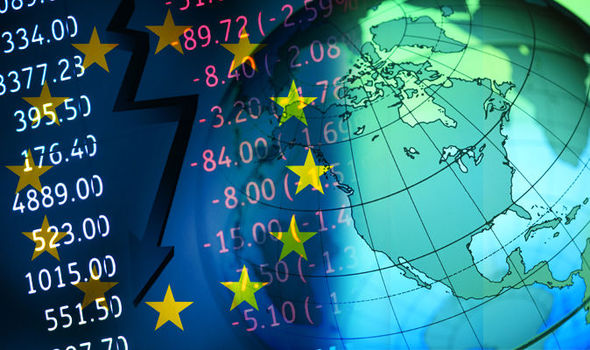
\includegraphics[width=\textwidth,height=0.5\textheight]{images/lesson01/fig3.jpg}

\hypertarget{principle-8-a-countrys-standard-of-living-depends-on-its-ability-to-produce-goods-services}{%
\section{Principle 8: A Country's Standard of Living Depends on Its Ability to Produce Goods \& Services}\label{principle-8-a-countrys-standard-of-living-depends-on-its-ability-to-produce-goods-services}}

\begin{itemize}
\tightlist
\item
  The most important determinant of living standards: \textbf{productivity}, the amount of goods and services produced per unit of labor.
\item
  Productivity depends on the equipment, skills, and technology available to workers.
\item
  Other factors (e.g., labor unions, competition from abroad) have far less impact on living standards.
\end{itemize}

\hypertarget{principle-9-prices-rise-when-the-government-prints-too-much-money}{%
\section{Principle 9: Prices Rise When the Government Prints Too Much Money}\label{principle-9-prices-rise-when-the-government-prints-too-much-money}}

\begin{itemize}
\tightlist
\item
  Inflation: increase in the general level of prices.
\item
  In the long run, inflation is almost always caused by excessive growth in the quantity of money, which causes the value of money to fall.
\item
  The faster the govt creates money, the greater the inflation rate.
\end{itemize}

\hypertarget{society-faces-a-short-run-tradeoff-between-inflation-and-unemployment}{%
\section{\texorpdfstring{\textbf{Principle 10:} Society Faces a Short-run Tradeoff Between Inflation and Unemployment}{ Society Faces a Short-run Tradeoff Between Inflation and Unemployment}}\label{society-faces-a-short-run-tradeoff-between-inflation-and-unemployment}}

\begin{itemize}
\tightlist
\item
  In the short-run (1--2 years), many economic policies push inflation and unemployment in opposite directions.
\item
  Other factors can make this tradeoff more or less favorable, but the tradeoff is always present.
\end{itemize}

\hypertarget{summary-triangleleft}{%
\section{\texorpdfstring{SUMMARY \(\triangleleft\)}{SUMMARY \textbackslash triangleleft}}\label{summary-triangleleft}}

\begin{enumerate}
\def\labelenumi{\arabic{enumi}.}
\tightlist
\item
  Because Resources are scarce, People Face Trade-offs
\item
  The Cost of Something Is What You Give Up to Get It
\item
  Rational People Think at the Margin
\item
  People Respond to Incentives
\item
  Trade Can Make Everyone Better Off
\item
  Markets Are Usually A Good Way to Organize Economic Activity
\item
  Governments Can Sometimes Improve Market Outcomes
\item
  A Country's Standard of Living Depends on Its Ability to Produce Goods \& Services
\item
  Prices Rise When the Government Prints Too Much Money
\item
  Society Faces a Short-run Tradeo Between In ation and Unemployment
\end{enumerate}

\hypertarget{principles-of-trade-and-interdependence-absolute-and-comparative-advantage}{%
\chapter{Principles of Trade and interdependence: Absolute and Comparative advantage}\label{principles-of-trade-and-interdependence-absolute-and-comparative-advantage}}

\hypertarget{learning-objectives-triangleleft}{%
\section{\texorpdfstring{Learning Objectives \(\triangleleft\)}{Learning Objectives \textbackslash triangleleft}}\label{learning-objectives-triangleleft}}

In this chapter, you will be able to answer the following:

\begin{itemize}
\item
  What are economists' two roles? How do they differ?
\item
  What are models? How do economists use them?
\item
  How is the \textbf{Production Possibilities Frontier (PPF)} related to opportunity cost? How does it help us understand gains from trade?
\item
  What is the difference between absolute and comparative advantage
\item
  What is the difference between positive and normative statement?
\end{itemize}

\hypertarget{what-do-economist-do}{%
\section{What do Economist Do?}\label{what-do-economist-do}}

\begin{itemize}
\item
  The two main roles of Economists:
\item
  Scientists: they try to explain the world
\item
  Policy advisers: try to improve the world
\item
  As scientists, economists employ the scientific method, objective development and testing of theories about how the world works.
\item
  Unlike the natural sciences, economists use mainly historical or survey data and less on lab experiments, which is difficult if not impossible in economics-- especially for the macroeconomy
\item
  As policy advisers, economists fight poverty, inflation, unemployment, etc.
\end{itemize}

\hypertarget{economists-as-scientists-assumptions-models}{%
\section{Economists as Scientists: Assumptions \& Models}\label{economists-as-scientists-assumptions-models}}

\begin{itemize}
\item
  As scientists, economists build \textbf{\emph{models}} to understand the world
\item
  \textbf{\emph{Model}}: a highly simplified representation of a reality.
\item
  we use \textbf{\emph{assumptions}} to simplify the complex world, make it easier to understand.
\item
  Example 1: To study int'l trade, we will assume two countries and two goods. Unrealistic, but simple to learn and gives useful insights about the real world.
\item
  Example 2: To understand relationship between two variables, it is often assumed that all other relevant factors remain unchanged, or ``other things equal'' or ceteris paribus in latin.
\end{itemize}

\hypertarget{example-model-the-production-possibilities-frontier}{%
\section{Example Model: The Production Possibilities Frontier}\label{example-model-the-production-possibilities-frontier}}

\begin{itemize}
\item
  The Production Possibilities Frontier (PPF): a graph that shows the combinations of two goods the economy can possibly produce given the available resources and the available technology
\item
  Example:
\end{itemize}

Two goods: computers and wheat

One resource: labor (measured in hours)

Economy has 50,000 labor hours per week available for production.

\hypertarget{ppf-example-complete-the-table-triangleleft}{%
\section{\texorpdfstring{PPF Example: Complete the table \(\triangleleft\)}{PPF Example: Complete the table \textbackslash triangleleft}}\label{ppf-example-complete-the-table-triangleleft}}

\begin{itemize}
\item
  Producing one computer requires 100 labor hours.
\item
  Producing one ton of wheat requires 10 labor hours.
\end{itemize}

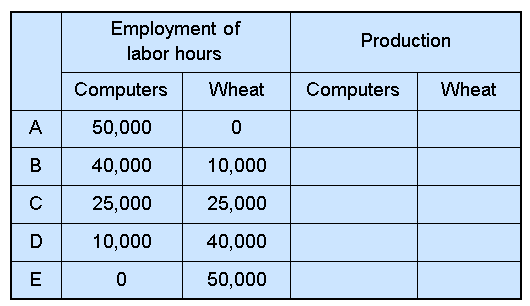
\includegraphics[width=\textwidth,height=0.6\textheight]{images/lesson02/page09.PNG}

\hypertarget{ppf-example-translate-to-graph-triangleleft}{%
\section{\texorpdfstring{PPF Example: Translate to graph \(\triangleleft\)}{PPF Example: Translate to graph \textbackslash triangleleft}}\label{ppf-example-translate-to-graph-triangleleft}}

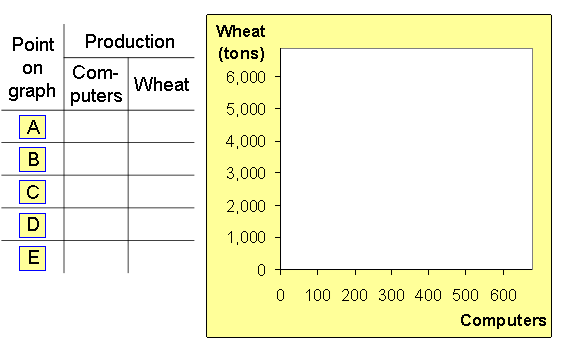
\includegraphics[width=\textwidth,height=0.75\textheight]{images/lesson02/page11.PNG}

\hypertarget{exercise-points-on-the-ppf}{%
\section{Exercise: Points on the PPF?}\label{exercise-points-on-the-ppf}}

\begin{enumerate}
\def\labelenumi{\alph{enumi}.}
\item
  On the graph, find the point that represents (100 computers, 3000 tons of wheat), label it \textbf{F}. Would it be possible for the economy to produce this combination of the two goods? Why or why not?
\item
  Next, find the point that represents (300 computers, 3500 tons of wheat), label it \textbf{G}. Would it be possible for the economy to produce this combination of the two goods?
\end{enumerate}

\hypertarget{the-ppf-and-opportunity-cost}{%
\section{The PPF and Opportunity Cost}\label{the-ppf-and-opportunity-cost}}

\begin{itemize}
\item
  The Opportunity Cost of good X
  \[= \frac{\textit{Additional amount of Y given up}}{\textit{Additional amount of X Obtained}} = |\frac{\Delta Y}{\Delta X} | = |slope|\]
\item
  Exercise: What is the Opportunity cost of producing Wheat for the previous PPF? and of Computer?
\end{itemize}

\hypertarget{active-learning-2-ppf-and-opprtunity-cost-triangleleft}{%
\section{\texorpdfstring{Active Learning 2: PPF and Opprtunity Cost \(\triangleleft\)}{Active Learning 2: PPF and Opprtunity Cost \textbackslash triangleleft}}\label{active-learning-2-ppf-and-opprtunity-cost-triangleleft}}

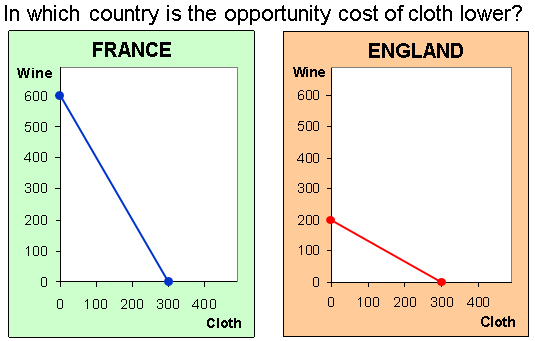
\includegraphics[width=\textwidth,height=0.5\textheight]{images/lesson02/page14.PNG}

\hypertarget{economic-growth-and-the-ppf}{%
\section{Economic Growth and the PPF}\label{economic-growth-and-the-ppf}}

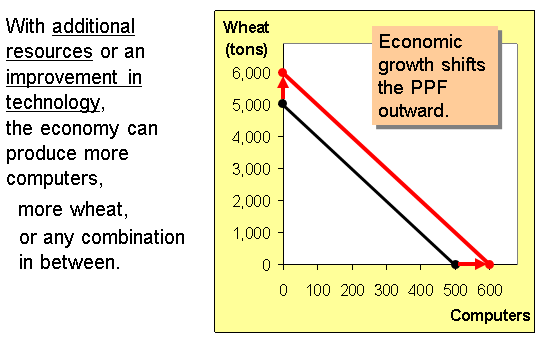
\includegraphics[width=\textwidth,height=0.5\textheight]{images/lesson02/page15.PNG}

\hypertarget{absolute-and-comparative-advantage}{%
\section{Absolute and Comparative Advantage:}\label{absolute-and-comparative-advantage}}

\hypertarget{first-example}{%
\subsection{First Example}\label{first-example}}

\begin{itemize}
\item
  Assumptions:
\item
  Two countries: the U.S. and the Rest of the World (RoW)
\item
  Two goods: computers and wheat
\item
  One resource: labor, measured in hours
\item
  We will look at how much of both goods each country produces and consumes
\item
  if the country chooses to be self-sufficient
\item
  if it trades with the other country
\item
  In U.S., Producing 1 computer requires 100 labor hours and
  Producing 1 ton of wheat requires 10 hours labor.
\item
  In the ROW, Producing 1 computer requires 90 labor hours and Producing 1 ton of wheat requires 15 hours labor.
\item
  Then:

  \begin{enumerate}
  \def\labelenumi{\alph{enumi}.}
  \item
    Which country is more efficient in the production of computers?
  \item
    Which country is more efficient in the production of wheat?
  \item
    So can U.S. gain from trade with ROW?
  \end{enumerate}
\end{itemize}

\textcolor{red}{\textbf{Absolute advantage:}}

\hypertarget{absolute-advantage}{%
\section{Absolute Advantage}\label{absolute-advantage}}

\begin{itemize}
\item
  \textcolor{red}{\textbf{Absolute advantage:}} the ability to produce a good using fewer inputs than another producer
\item
  Which country has an absolute advantage in computers?
\item
  Which country has an absolute advantage in wheat?
\end{itemize}

\hypertarget{another-example-u.s.-japan-triangleleft}{%
\section{\texorpdfstring{Another Example: U.S. \& Japan \(\triangleleft\)}{Another Example: U.S. \& Japan \textbackslash triangleleft}}\label{another-example-u.s.-japan-triangleleft}}

\begin{itemize}
\item
  U.S. again has 50,000 hours of labor per month available for production.
\item
  Producing 1 computer requires 100 hours of labor. Producing 1 ton of wheat requires 10 hours of labor.
\item
  Japan has also 50,000 hours of labor available for production, per month.
\item
  Producing 1 computer requires 125 hours of labor. Producing 1 ton of wheat requires 25 hours of labor.
\item
  Which country has absolute adv. in the production of wheat? in the production of computers? Can U.S. benefit in trade with Japan?
\end{itemize}

\hypertarget{u.s-and-japan-without-trade-triangleleft}{%
\section{\texorpdfstring{U.S and Japan without Trade \(\triangleleft\)}{U.S and Japan without Trade \textbackslash triangleleft}}\label{u.s-and-japan-without-trade-triangleleft}}

\begin{itemize}
\tightlist
\item
  Suppose U.S. allocates its resources 50-50 to each good, while Japan allocates 1/4 on computers and 3/4 on wheat. Locate this in each country's PPF. (Without trade each country consumes what it produces, no more no less!)
\end{itemize}

\centering

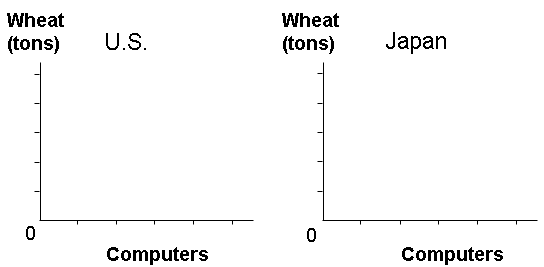
\includegraphics[width=\textwidth,height=0.75\textheight]{images/lesson02/part2/page18.PNG}

\hypertarget{active-learning-triangleleft}{%
\section{\texorpdfstring{\emph{Active Learning:} \(\triangleleft\)}{Active Learning: \textbackslash triangleleft}}\label{active-learning-triangleleft}}

\begin{itemize}
\item
  If U.S. specializes only in computers, what is the maximum number of computers it can produce? locate this point on the U.S. PPF.
\item
  Suppose Japan produces only 400 computers. How many tons of wheat would Japan be able to produce with its remaining labor? Draw this point on Japan's PPF.
\end{itemize}

\hypertarget{basic-international-trade-terms}{%
\section{Basic International Trade Terms}\label{basic-international-trade-terms}}

\begin{itemize}
\item
  \textcolor{red}{\textbf{Exports: }} goods produced domestically and sold abroad
\item
  \textbf{To export} means to sell domestically produced goods abroad.
\item
  \textcolor{red}{\textbf{Imports: }} goods produced abroad and sold domestically
\item
  \textbf{To import} means to purchase goods produced in other countries.
\end{itemize}

\hypertarget{activity-consumption-with-trade-triangleleft}{%
\section{\texorpdfstring{Activity: Consumption With Trade \(\triangleleft\)}{Activity: Consumption With Trade \textbackslash triangleleft}}\label{activity-consumption-with-trade-triangleleft}}

Suppose the U.S. exports 2000 tons of wheat to Japan, and imports 280 computers from Japan.

\bigskip

(So, Japan imports 2000 tons wheat and exports 280 computers. The rate of exchange is called terms of trade)

\begin{itemize}
\item
  How much of each good is consumed in the U.S.? Plot this combination on the U.S. PPF.
\item
  How much of each good is consumed in Japan?
\end{itemize}

Plot this combination on Japan's PPF.

\hypertarget{u.s.-production-and-consumption-with-trade-triangleleft}{%
\section{\texorpdfstring{U.S. Production and Consumption With Trade \(\triangleleft\)}{U.S. Production and Consumption With Trade \textbackslash triangleleft}}\label{u.s.-production-and-consumption-with-trade-triangleleft}}

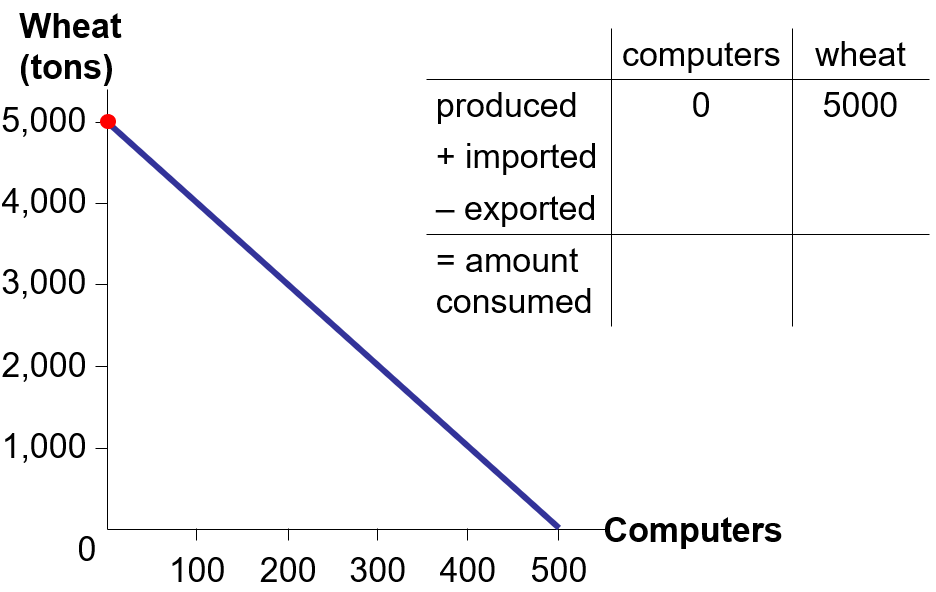
\includegraphics[width=\textwidth,height=0.75\textheight]{images/lesson02/part2/page19.PNG}

\hypertarget{japans-production-and-consumption-with-trade-triangleleft}{%
\section{\texorpdfstring{Japan's production and Consumption With Trade \(\triangleleft\)}{Japan's production and Consumption With Trade \textbackslash triangleleft}}\label{japans-production-and-consumption-with-trade-triangleleft}}

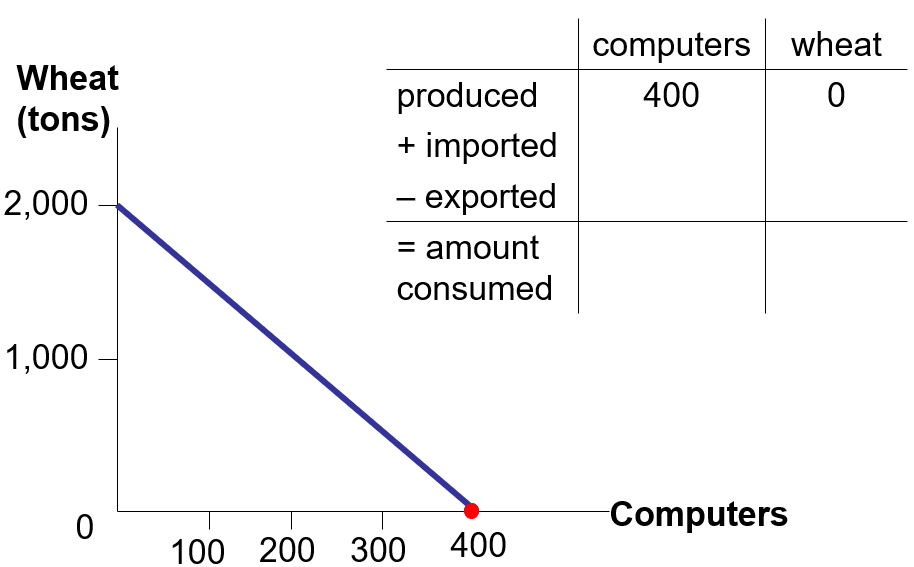
\includegraphics[width=\textwidth,height=0.75\textheight]{images/lesson02/part2/page20.PNG}

\hypertarget{trade-makes-both-countries-better-off-triangleleft}{%
\section{\texorpdfstring{Trade Makes Both Countries Better Off \(\triangleleft\)}{Trade Makes Both Countries Better Off \textbackslash triangleleft}}\label{trade-makes-both-countries-better-off-triangleleft}}

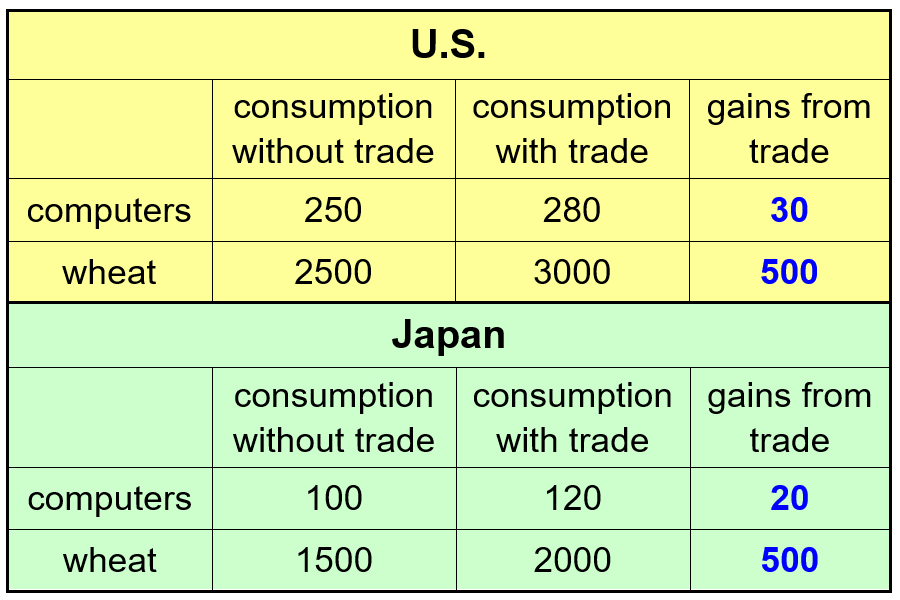
\includegraphics[width=\textwidth,height=0.75\textheight]{images/lesson02/part2/page21.PNG}

\textcolor{red}{\textbf{Comparative Advantage:}}

\hypertarget{where-do-these-gains-come-from}{%
\section{Where Do These Gains Come From?}\label{where-do-these-gains-come-from}}

\begin{itemize}
\item
  So, the U.S. has an absolute advantage in both goods but can again from trade with Japan!
\item
  why does Japan specialize in computers? Why do \underline{both} countries gain from trade?
\item
  Or can absolute advantage explain the possibility of trade between the countries?
\end{itemize}

\hypertarget{opportunity-cost-and-comparative-advantage}{%
\section{Opportunity Cost and Comparative Advantage}\label{opportunity-cost-and-comparative-advantage}}

\begin{itemize}
\item
  Recall: Another measure of cost is opportunity cost.
\item
  \textbf{\emph{Comparative advantage:}} the ability to produce
\end{itemize}

a good at a lower opportunity cost than another producer

\begin{itemize}
\item
  Which country has the comparative advantage in computers?
\item
  Which country has the comparative advantage in wheat?
\end{itemize}

\bigskip

\textbf{\emph{Lesson}}: Absolute advantage is not necessary for comparative advantage or for trade! Comparative advantage is!

\hypertarget{comparative-advantage-and-trade}{%
\section{Comparative Advantage and Trade}\label{comparative-advantage-and-trade}}

\begin{itemize}
\item
  Gains from trade arise from comparative advantage (differences in opportunity costs).
\item
  Specialization and trading according to comparative advantage increases world production and consumption. (each country still produce on its PPF but can consume combinations outside its PPF)
\item
  The same applies to individual producers (like the farmer and the rancher) specializing in different goods and trading with each other.
\end{itemize}

\hypertarget{active-learning-1-absolute-comparative-advantage}{%
\section{\texorpdfstring{\emph{Active Learning 1: Absolute \& comparative advantage}}{Active Learning 1: Absolute \& comparative advantage}}\label{active-learning-1-absolute-comparative-advantage}}

\begin{itemize}
\item
  Argentina and Brazil each have 10,000 hours of labor per month.
\item
  In Argentina:

  \begin{itemize}
  \tightlist
  \item
    producing one pound coffee requires 2 hours
  \item
    producing one bottle wine requires 4 hours
  \end{itemize}
\item
  In Brazil:

  \begin{itemize}
  \tightlist
  \item
    producing one pound coffee requires 1 hour
  \item
    producing one bottle wine requires 5 hours
  \end{itemize}
\end{itemize}

\begin{enumerate}
\def\labelenumi{\alph{enumi}.}
\item
  Which country has an absolute advantage in the production of coffee ?
\item
  Which country has a comparative advantage in the production of wine?
\end{enumerate}

\hypertarget{active-learning-2-absolute-comparative-advantage-triangleleft}{%
\section{\texorpdfstring{\emph{Active Learning 2: Absolute \& comparative advantage} \(\triangleleft\)}{Active Learning 2: Absolute \& comparative advantage \textbackslash triangleleft}}\label{active-learning-2-absolute-comparative-advantage-triangleleft}}

images/lesson02/part2/page23a.PNG)\{height=75\%\}

\small

Assuming each worker has only 8 hours daily for production:

\begin{enumerate}
\def\labelenumi{\alph{enumi}.}
\item
  Who has absolute advantage in the production of jackets? ties?
\item
  Who has comp. advantage in the production of jackets? ties?
\item
  Suppose the terms of trade were 1 jacket to 2 ties, show how each person is made better off through specialization and trade
\end{enumerate}

\hypertarget{active-learning-3-absolute-comparative-advantage-triangleleft}{%
\section{\texorpdfstring{\emph{Active Learning 3: Absolute \& comparative advantage} \(\triangleleft\)}{Active Learning 3: Absolute \& comparative advantage \textbackslash triangleleft}}\label{active-learning-3-absolute-comparative-advantage-triangleleft}}

\begin{itemize}
\item
  Germany can produce 2 computers per minute or 1 tractor per minute while the U.S. can produce 3 computers of 2 tractors per minute. Draw the implied PPF and show:

  \begin{enumerate}
  \def\labelenumi{\alph{enumi}.}
  \item
    Which country has absolute advantage in computers? in tractors?
  \item
    Which country has comp. advantage in computers? in tractors?
  \item
    what is the range in which trade can benefit both countries.
  \end{enumerate}
\end{itemize}

\hypertarget{active-learning-4-absolute-comparative-advantage-diamond}{%
\section{\texorpdfstring{\emph{Active Learning 4: Absolute \& comparative advantage} \(\diamond\)}{Active Learning 4: Absolute \& comparative advantage \textbackslash diamond}}\label{active-learning-4-absolute-comparative-advantage-diamond}}

Assume that England and Spain can switch between producing cheese and producing bread at a constant rate.

images/lesson02/part2/img01\_Engl.PNG)\{height=100\%\}

\begin{enumerate}
\def\labelenumi{\alph{enumi}.}
\item
  Which country has absolute advantage in Cheese? in bread?
\item
  Which country has comp. advantage in Cheese? in bread?
\end{enumerate}

\hypertarget{unanswered-questions}{%
\section{\texorpdfstring{Unanswered Questions \ldots }{Unanswered Questions }}\label{unanswered-questions}}

\begin{itemize}
\item
  We made a lot of assumptions about the quantities of each good that each country produces, trades, and consumes, and the price at which the countries trade wheat for computers.
\item
  In the real world, these quantities and prices would be determined by the preferences of consumers and the technology and resources in both countries.
\item
  We will begin to study this in the next chapter. For now, though, our goal was merely to see how \textcolor{blue}{trade can make everyone better off.}
\end{itemize}

\hypertarget{chapter-summary}{%
\section{CHAPTER SUMMARY}\label{chapter-summary}}

\begin{itemize}
\item
  Interdependence and trade allow everyone to enjoy a greater quantity and variety of goods \& services.
\item
  Comparative advantage means being able to produce a good at a lower opportunity cost. Absolute advantage means being able to produce a good with fewer inputs.
\item
  When people -- or countries -- specialize in the goods in which they have a comparative advantage, the economic ``pie'\,' grows and trade can make everyone better off.
\end{itemize}

\hypertarget{the-economist-as-policy-advisor}{%
\section{The Economist as Policy Advisor}\label{the-economist-as-policy-advisor}}

\begin{itemize}
\item
  As scientists, economists make \textcolor{red}{\textbf{positive statements,}} which attempt to describe the world as it is.
\item
  As policy advisors, economists make \textcolor{red}{\textbf{normative statements,}} which attempt to prescribe how the world should be.
\item
  Positive statements can be confirmed or refuted, normative statements cannot.
\end{itemize}

\hypertarget{active-learning-identifying-positive-vs.-normative-triangleleft}{%
\section{\texorpdfstring{\textbf{\emph{ACTIVE LEARNING: Identifying positive vs.~normative}} \(\triangleleft\)}{ACTIVE LEARNING: Identifying positive vs.~normative \textbackslash triangleleft}}\label{active-learning-identifying-positive-vs.-normative-triangleleft}}

Which of these statements are ``positive'' and which are ``normative''? How can you tell the difference?

\begin{enumerate}
\def\labelenumi{\alph{enumi}.}
\item
  Prices rise when the government increases the quantity of money.
\item
  The government should print less money.
\item
  A tax cut is needed to stimulate the economy.
\item
  An increase in the price of burritos will cause an increase in consumer demand for video rentals.
\end{enumerate}

\hypertarget{why-economists-disagree}{%
\section{Why Economists Disagree}\label{why-economists-disagree}}

Economists sometimes give conflicting policy advice.

\begin{itemize}
\item
  They sometimes disagree about the validity of alternative positive theories about the world.
\item
  They may have different values and, therefore, different normative views about what policy should try to accomplish.
\end{itemize}

Yet, there are many propositions about which most economists agree.

\hypertarget{propositions-about-which-most-economists-agree-and-who-agree}{%
\section{Propositions about Which Most Economists Agree (and \% who agree)}\label{propositions-about-which-most-economists-agree-and-who-agree}}

\begin{itemize}
\item
  A ceiling on rents reduces the quantity and quality of housing available. (93\%)
\item
  Tariffs and import quotas usually reduce general economic welfare. (93\%)
\item
  The United States should not restrict employers from outsourcing work to foreign countries. (90\%)
\item
  The United States should eliminate agriculture subsidies. (85\%)
\end{itemize}

\hypertarget{fyi-who-studies-economics}{%
\section{FYI: Who Studies Economics?}\label{fyi-who-studies-economics}}

\begin{itemize}
\tightlist
\item
  Tiger Woods, Golfer
\item
  Ronald Reagan, President of the United States
\item
  Barbara Boxer, U.S. Senator
\item
  Sandra Day-O'Connor, Former Supreme Court Justice
\item
  Anthony Zinni, Former General, U.S. Marine Corps
\item
  Kofi Annan, Former Secretary General, United Nations
\item
  Meg Witman, Chief Executive Officer, eBay
\item
  Steve Ballmer, Chief Executive Officer, Microsoft
\item
  Arnold Schwarzenegger, Governor of California, Actor
\item
  Ben Stein, Political Speechwriter, Actor, Game Show Host
\item
  Mick Jagger, Singer for the Rolling Stones
\item
  John Elway, NFL Quarterback
\item
  Diane von Furstenburg, Fashion Designer
\end{itemize}

\hypertarget{chapter-summary-1}{%
\section{CHAPTER SUMMARY}\label{chapter-summary-1}}

\begin{itemize}
\item
  As scientists, economists try to explain the world using models with appropriate assumptions.
\item
  Two simple models are the Circular Flow Diagram and Production Possibilities Frontier.
\item
  As policy advisers, economists offer advice on how to improve the world.
\end{itemize}

\end{document}
